\documentclass{egpubl}
\usepackage{gg2022}

\ConferencePaper      % uncomment for (final) Conference Paper

\title[Visualization of relativity]{Visualization of relativistic phenomena}

\author{Zoltán Simon}

\usepackage[pdftex]{graphicx} \pdfcompresslevel=9
\usepackage{t1enc,dfadobe}
\usepackage{amsmath}
\usepackage{placeins}

% For backwards compatibility to old LaTeX type font selection.
% Uncomment if your document adheres to LaTeX2e recommendations.
\let\rm=\rmfamily    \let\sf=\sffamily    \let\tt=\ttfamily
\let\it=\itshape     \let\sl=\slshape     \let\sc=\scshape
\let\bf=\bfseries

% if the Editors-in-Chief have given you the data, you may uncomment
% the following five lines and insert it here
%
% \volume{22}   % the volume in which the issue will be published;
% \issue{3}     % the issue number of the publication
% \pStartPage{???}      % set starting page


\begin{document}

\maketitle

\begin{abstract}
Special relativity describes many phenomena, not observable in everyday life. This article presents an educational application, which helps to understand these effects. It models vision of objects travelling close to the speed of light. e. g. it visualizes length contraction, time dilatation, relativistic Doppler effect. It considers the path of light between the object and our eye, but it also presents an opportunity to visualize events happening simultaneously as well. It allows to switch between Lorentz and Galilean transformation, so we can compare Einstein's and Newton's model. It serves with a three-dimensional space-time diagram, on which we have a chance to further analyse the movement of objects.
\end{abstract}

\section{Introduction}
\label{sec:introduction}
Theory of relativity is a key part of modern physics. There are many use cases of this theory. Despite of it's importance there is very little chance for people to experience relativistic phenomena in their everyday life, thus differences between Isaac Newton's classical and Albert Einstein's modern model remain unexplored. The application described in this article offers a way to visualise the most well-known phenomena associated with special relativity. The goal of this article is to showcase the algorithmic challenges surrounding this program and introduce solutions for these problems.

\section{Theoretical background}
\label{sec:theoretical_background}
The rules of simulation are based on Einstein's postulates~\cite{EinsteinElectrodynamics}. These suggest that
\begin{itemize}
\item an observer can not differentiate between different inertial frames of reference by taking measurements in each frame of reference.
\item the velocity of propagation of any physical effect can not exceed
the speed of light in vacuum: $c=299792458 \frac{m}{s} \sim 3 \cdot 10^8 \frac{m}{s}$.
 \end{itemize}
These two constraints do not provide sufficient tools for the programmer on their own. However, all the required formulas can be derived from these two postulates.

\subsection{Usage of the term ,,absolute frame''}
To simplify representation of world lines every event and velocity is described in the same frame of reference. In code this frame of reference is called absolute frame. This helps circumvent confusion when transforming between different observer's proper frames. Each value is stored as it is measured in absolute frame. When visualising a given value, than it gets transformed to a particular observers proper frame.

\subsection{Representation of physical bodies}
To model the journey of physical objects through space-time, it is convenient to assign a world line to each object. To be more precise, this is going to be the world line of the object's origin point. For practical purposes this point is selected to be the same as the origin point in model space. Such world line can be stored as a set of events. We assume geodetic world line between two neighbouring events. At this point it is necessary to note, that we also assume flat space-time. This method allows us to represent world lines consisting of few geodetic sections easily. World lines of accelerating objects appear curved in space-time diagrams. We can approximate these lines by a set of short geodetic sections. This approximation is useful, because along the small sections we can use the simple formulas of Lorentz transformation. The downside of this method is, that many calculations require iteration over the small sections. E. g. determining the age of an object without a priory information requires summing of ageing of the object along the geodetic sections. The other obvious downside of such approximation is, that the resulting world line is going to have relatively low resolution. This is particularly noticeable, when we --as a viewer-- place ourselves in the proper frame of such accelerating object. In this case the violent jumping nature of the movement of surroundings is much more noticeable.

\section{View modes}
The application supports multiple view modes. The two main modes are the \emph{real time} three dimensional view and the \emph{diagram view}. In the \emph{real time} mode the scene is shown as regular three dimensional scene, changing over time. We can look around with the virtual camera to observe the moving objects. The shape and colour of objects gets distorted in accordance with the relativistic effects. 

In the \emph{diagram view} we can observe the world lines of objects present in the scene. This provides additional insight into the behaviour of objects. As a recent addition to the project now the user can switch to orthographic projection from the standard perspective projection. This improves the readability of the space-time diagram, and it's also useful in the \emph{real time} view.

In order to help the user spot differences between classic and relativistic physics, there is a way to switch between Galilean \cite{KHGalilei} and Lorentz transformation. A viewer can see the incoming light from an object, thus we can only see images showing the past. This is due to the finiteness of the speed of light. The application allows to toggle between visualisation of present event as described in the selected observer's frame, and past events in accordance with the incoming light beams.

\subsection{Switching between observers}
To compare the observations in different inertial frames of reference, we can toggle between multiple observers. In this implementation observers are independent from physical objects, however it's possible to make an observer follow an object. Every observer has it's own world line. These lines are also visible in \emph{diagram view}.

When switching between frames of reference the origin of the frame also changes. The $\vec{O} =(0,0,0)$ in currently selected proper frame gets assigned to the space coordinate vector of an event along the world line of the observer. The question is, how do we select the time component. In other words which event will be selected along the new world line. This implementation chooses the event from the new observers world line, which happened simultaneously whit the event of changing observers according to the previous observer. This method introduces a somewhat more realistic approach, however in real life still no object can travel from one event's location to an other's if these two events appear to be simultaneous. This would require velocity greater than the speed of light. In defence of this approach in this computer simulation neither the user's perspective nor an observer is necessary bound to a physical object. At least this way the false sense, that the \emph{absolute frame} in the program would have special characteristics in real life is weakened.

\subsection{Visualisation of simultaneous events}
\label{visOfSimEvents}
The less realistic approach for selecting events to render takes the simultaneously happening events. Luckily present events form a hyperplane in the four dimensional space-time. Present events along object's world lines can be obtained by calculating intersections between the world lines and this simultaneous hyperplane. The hyperplane can be described by an event and a normal four-vector. The event is going to be the one along the world line associated with the observer, of which time component is $t_{abs}$~time~variable of the simulation. The normal vector is obtained from the $\vec{v}=(v_x, v_y, v_z, v_t)$ velocity of the observer's frame relative to the \emph{absolute frame}. This is described in form \ref{normalOfSimult}.
\begin{equation}
\vec{n}_{pl} = (-v_x, -v_y, -v_z, v_t)
\label{normalOfSimult}
\end{equation}

Equation \ref{planeIntersection} for calculating the intersection between the line and plane is analogous to the one used in three dimensional space, where $\vec{n}_{pl}$ is the normal of the hyperplane, $\vec{p}_{pl}$ is the event on the plane, $\vec{s}_{wl}$ is a starting event of the geodetic world line and $\vec{v}_{wl}$ is the velocity four-vector of the this world line. Note that the resulting $t$ parameter is not the time measured by the object travelling along the world line nor the time measured in the \emph{absolute frame}. This is simply a ray parameter, although can be easily transformed to the time measured in \emph{absolute frame} by multiplying by the time component of $\vec{v}_{wl}$ four-velocity.
\begin{equation}
\label{planeIntersection}
t = \frac{\vec{n}_{pl}\cdot(\vec{p}_{pl} - \vec{s}_{wl})}{\vec{v}_{wl}\cdot\vec{n}_{pl}}
\end{equation}

The previously described equation can handle geodetic world lines. To use this with segmented world lines we need to iterate over the small geodetic segments. 

\subsection{Visualisation of events considering the propagation of light}
\label{visConsLight}
A more realistic approach for finding events to render uses the event horizon as the intersecting hypersurface. From greater distances older events are seen. This characteristic makes the event horizon analogous with a cone in three dimensional space. The  event describing the position and age of the viewer is enough to describe this hypercone. The quadratic equation~\ref{eq:coneIntersection} provides the tool for calculating the intersection.
\begin{align}
a &= v_x^2 + v_y^2 + v_z^2 - v_t^2\\
\vec{m} &= (s_x, s_y, s_z)\cdot{}(v_x, v_y, v_z) - (v_x, v_y, v_z)\cdot{}(c_x, c_y, c_z)\\
b &= 2((m_x + m_y + m_z) - (s_t\cdot{}v_t - v_t\cdot{}c_t))\\
c &= ((c_x, c_y, c_z) - (s_x, s_y, s_z))\cdot{}((c_x, c_y, c_z) - (s_x, s_y, s_z))\\
0 &=ax^2 + bx + c
\label{eq:coneIntersection}
\end{align}

Because no world line can exceed the speed of light, the roots of the equation are always going to be real values. We select the root associated with the past event. 

When using Galilean transformation, the hypercone could have different shapes in different frames of reference. This is because the speed of light is not measured to be equal in all frames of reference. This implementation tackles this problem by considering the \emph{absolute frame} the one, where speed of light equals to $c$ in any random direction. This is convenient from computational standpoint, because the program works with values represented in this frame of reference anyway.

\section{Rendering pipeline in real time mode}
Let's take a closer look at the path taken by the data describing an object until it appears on screen. We focus on the \emph{real time} mode, because in \emph{diagram view} the world line of an object explicitly gets converted to a line in three dimensional space by removing one space coordinate and using the time component instead. However in \emph{real time} mode more calculation is required.

We need to calculate separate world line for each vertex of a geometry. Because of the spacial differences between different points of an object, they tend to behave significantly different. Consequently the shape of an object gets distorted. For this to behave somewhat realistically, high resolution meshes are required. Even a cube hast to be composited from many polygons. The program was tested with cube geometry consisting of 12300 polygons, 36900 vertices. This makes possible, that the edges of a cube appear curved when transformed.

\subsection{Generating world lines for vertices with relativistic procedure}
\label{sec:genRelProc}
First step in generating the world line for a given vertex is determining the $s$ starting event of the world line. This is done by taking the spacial coordinates of the vertex modified by the length contraction formula \ref{lengthContraction} and appending these with a $0$ as the time component. This is interpreted as an event that is at the intersection of the simultaneous hyperplane of the \emph{absolute frame} at $t = 0 m$ and this world line. The length contraction is applied in the direction of the velocity of the object relative to the \emph{absolute frame}.
\begin{equation}
\label{lengthContraction}
l' =l\sqrt{1 - \frac{v^2}{c^2}}
\end{equation}

By taking the initial $\vec{v}_0$ four-velocity of the object's origin's world line and our new $\vec{s}$ starting event, we get the first geodetic segment of the new world line. The next step is to calculate the ending event of this section. In this implementation we assume, that all vertices of the object get boosted simultaneously with the origin of the object. Simultaneity is determined in the proper frame of the object prior to the event of the boost. Thus, the ending event is the intersection between the mentioned simultaneous hyperplane and the geodetic world line segment. This method is able to recreate \emph{Wigner rotation} as described in section~\ref{sec:wigner_rotation}. The ending event of the current segment will be the starting event of the following event. Please note, that this method introduces an accumulated error to the iteration caused by the computer's finite precision of number representation. The velocity is always equal to the origin point's velocity in the corresponding segment. Before the first starting event and after the last ending event the algorithm assumes, that the first  and last segment is a continuation and is continued by the same geodetic world line respectively.

During the previously described iteration intersection between the hyperplane or hypercone and the segments can be obtained as described in sections \ref{visOfSimEvents} and \ref{visConsLight}. As an optimization the iteration can be quit after this intersection is found.

The finishing steps of the rendering pipeline include transforming the found intersection event from the \emph{absolute frame} to the proper frame of the current observer using the \emph{Lorentz transformation} and calculating the \emph{Doppler shift} of colour. When calculating the \emph{Doppler shift} the relative velocity between the selected observer and the object's proper frame also must be transformed with the \emph{Lorenty transformation} for velocity.

\subsection{Generating world lines for vertices with classic procedure}
When using the \emph{Galilean transformation}, generating world lines for the vertices is similar to the one described in subsection~\ref{sec:genRelProc}. The key differences are described in this subsection. When creating the $\vec{s}$ starting event for the world line, no length contraction is applied. The ending event of segments can be obtained by translating the events of the object's origin's world line by the spacial coordinates of the vertex. This way we also eliminate the accumulated error introduced by the method in \ref{genRelProc}. This simplification is available, because in Newton's model simultaneity is absolute, thus events of boosting have equal time component.

After obtaining the intersection event between the hyperplane or hypercone and the world line of a vertex, \emph{Galilean transformation} is applied, to obtain the coordinates of the event in the selected observers proper frame and the relative velocity between the object's and observer's proper frame.

\section{Wigner rotation}
\label{sec:wigner_rotation}
I this section we take a closer look at the details of Wigner rotation and it's implementation in the simulator. <Work in progress>\dots

\section{Results}
\label{sec:results}
This section showcases the images renderer by this application. These images focus on a selection of popular relativistic phenomena.

When an object passes by in front of the viewer, the object appears to be rotated. The rotation axis is perpendicular to the movement direction and the viewer's direction from the object. This is shown in Figure~\ref{fig:RotatingDice}. Top dice is moving to left in parallel with the viewing plane. The effect is the consequence of light beams travelling different distances from different points of the object.

\begin{figure}[h]
\center
\resizebox{70mm}{!}{
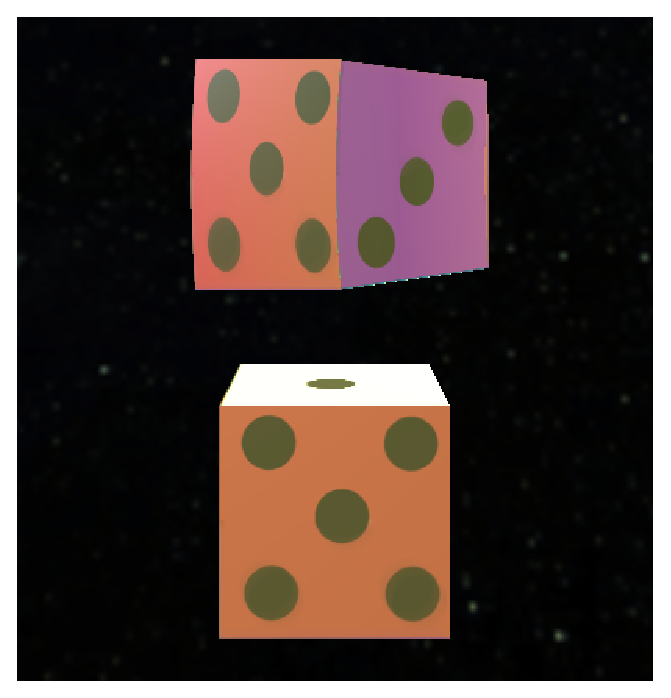
\includegraphics{figures/rotatingDice.eps}
}
\caption{Rotating dice}
\label{fig:RotatingDice}
\end{figure}

If we ignore the path travelled by photons towards the eye, than simultaneous events can be seen. This way the length contraction is observable as shown in Figure~\ref{fig:lengthContraction}.

\begin{figure}[h]
\center
\resizebox{70mm}{!}{
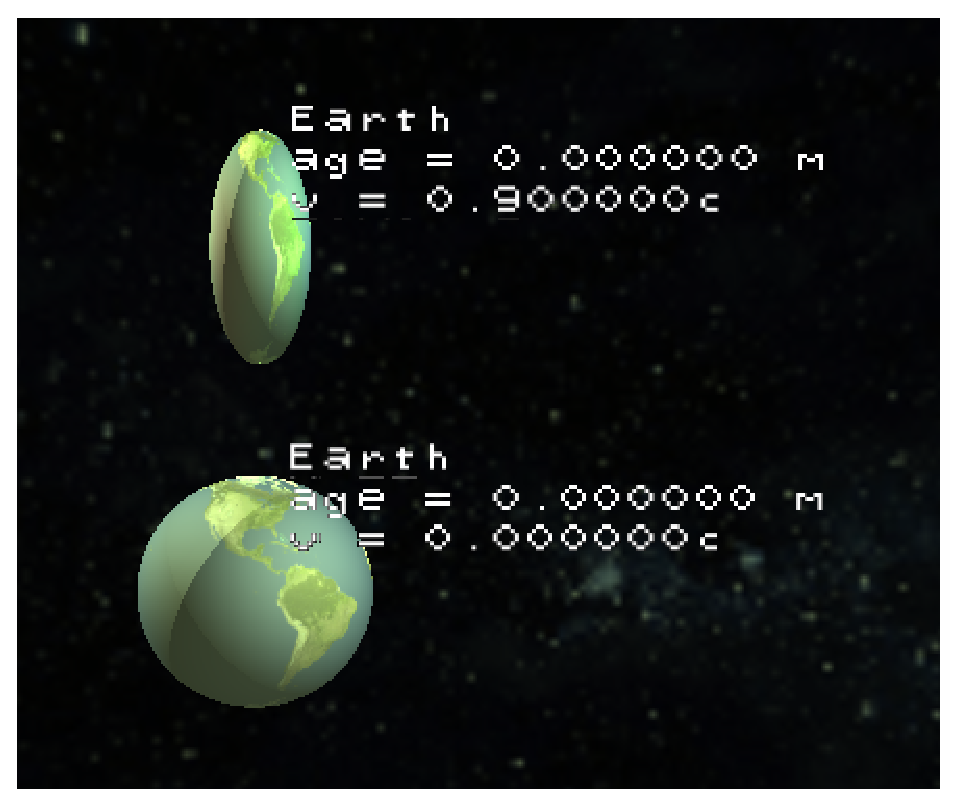
\includegraphics{figures/lengthContraction.eps}
}
\caption{Length contraction}
\label{fig:lengthContraction}
\end{figure}

The twin paradox as described by Albert Einstein can be demonstrated in \emph{diagram view}. This is seen in Figure~\ref{fig:twinParadox}.

\begin{figure}[h]
\center
\resizebox{70mm}{!}{
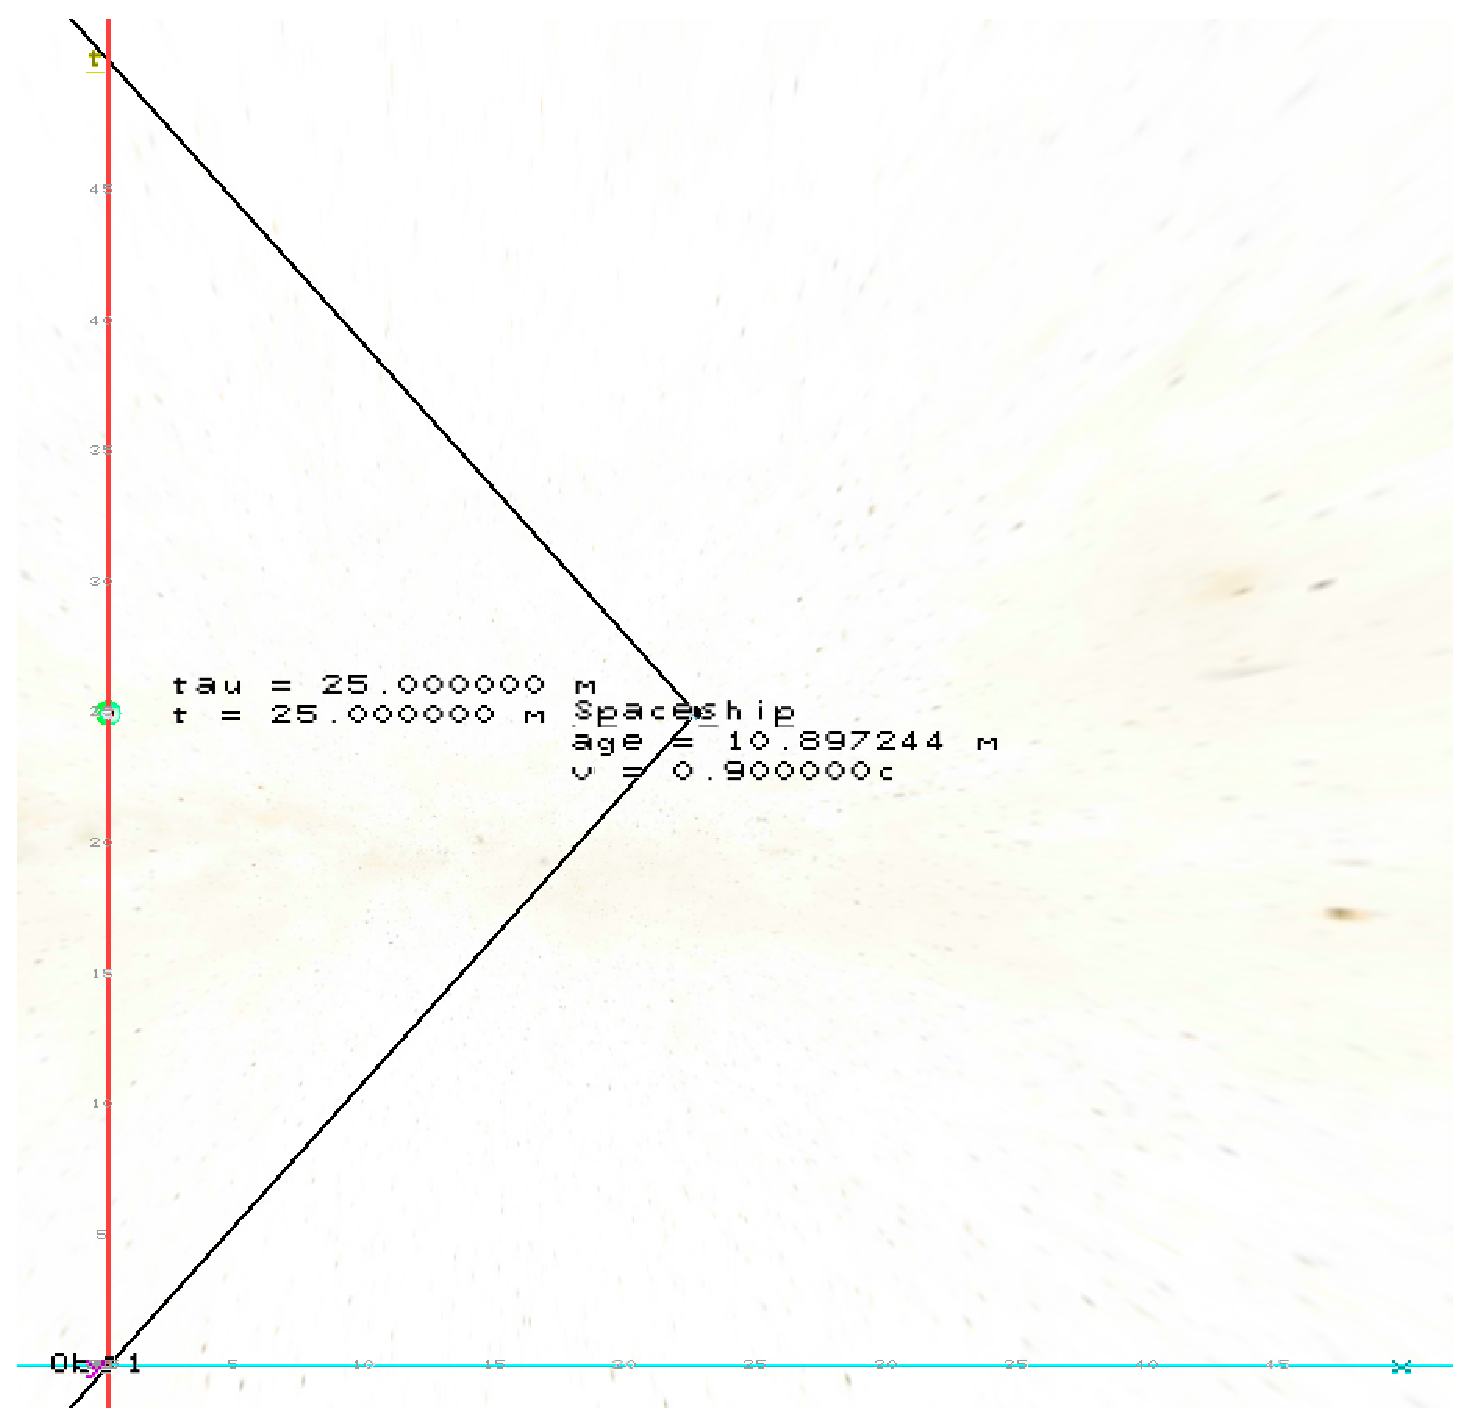
\includegraphics{figures/twinParadox.eps}
}
\caption{Twin paradox}
\label{fig:twinParadox}
\end{figure}

Take a look at the world lines of objects following circular trajectory. 
In Figure~\ref{fig:circularWL}, the lines appear, to be wound up around the time axis.

\begin{figure}[h]
\center
\resizebox{70mm}{!}{
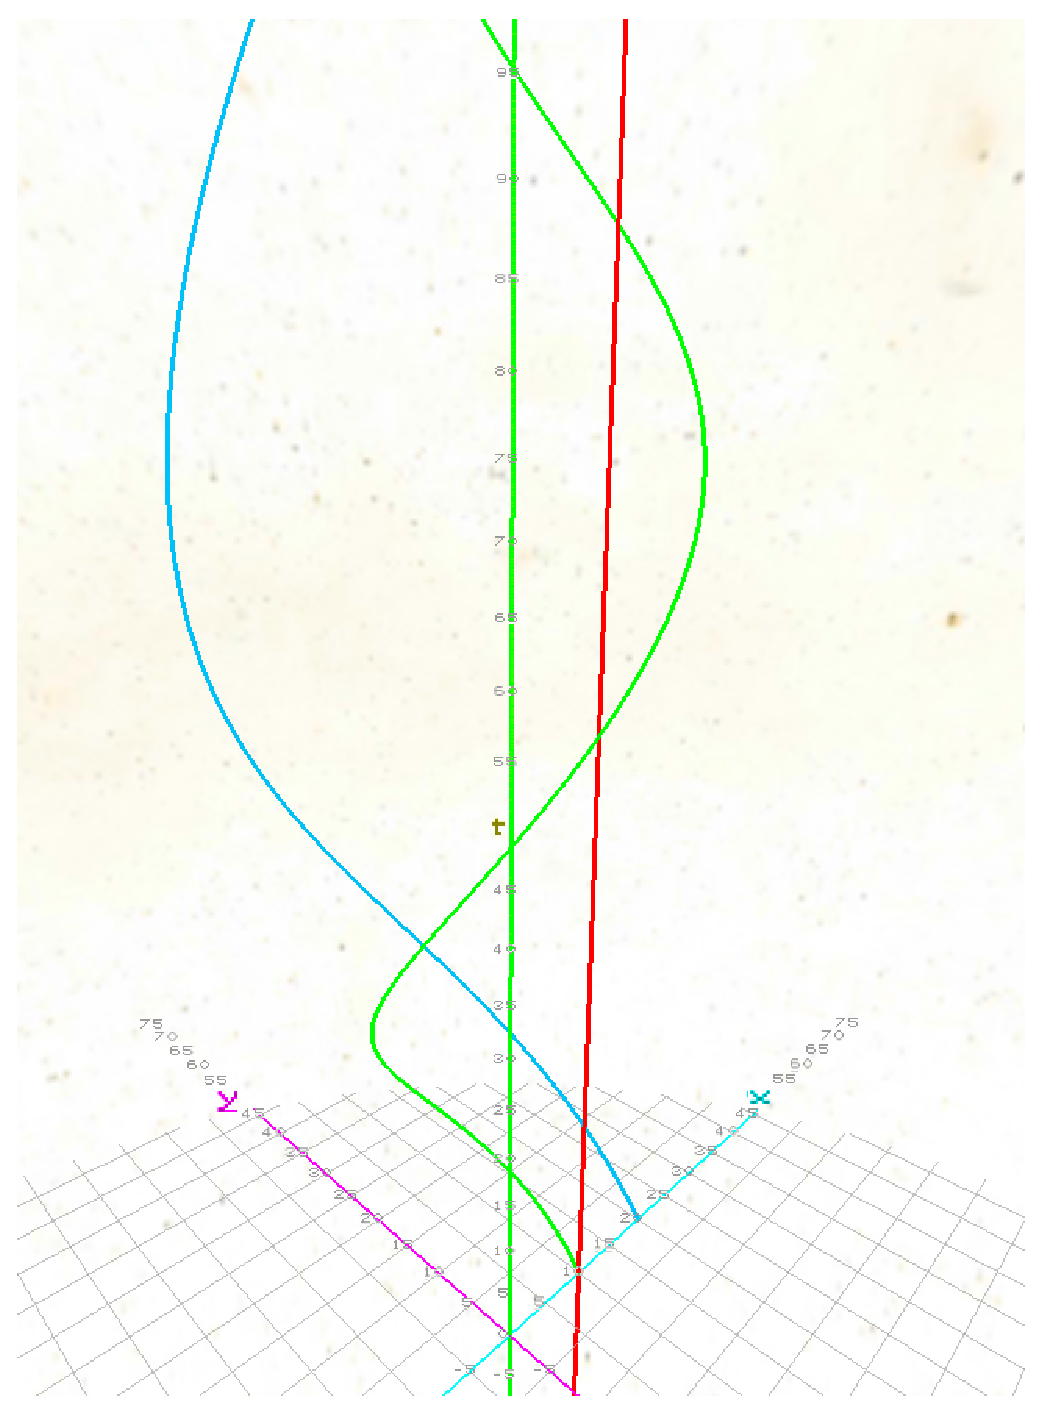
\includegraphics{figures/circularWL.eps}
}
\caption{Circular world line}
\label{fig:circularWL}
\end{figure}

When we switch to \emph{real time} mode, than we can observe the Thomas precession of the circulating object. This can be seen in Figure~\ref{fig:thomasPrec}. The object on the left is standing in the observer's frame. The right object is moving along a circular path. The path has radius of $r=20m$, and the tangential velocity of the object is $v=0,8$
The time of the full rotation according the observer was $T=167m$.
\begin{figure}[htb]
  	\centering
	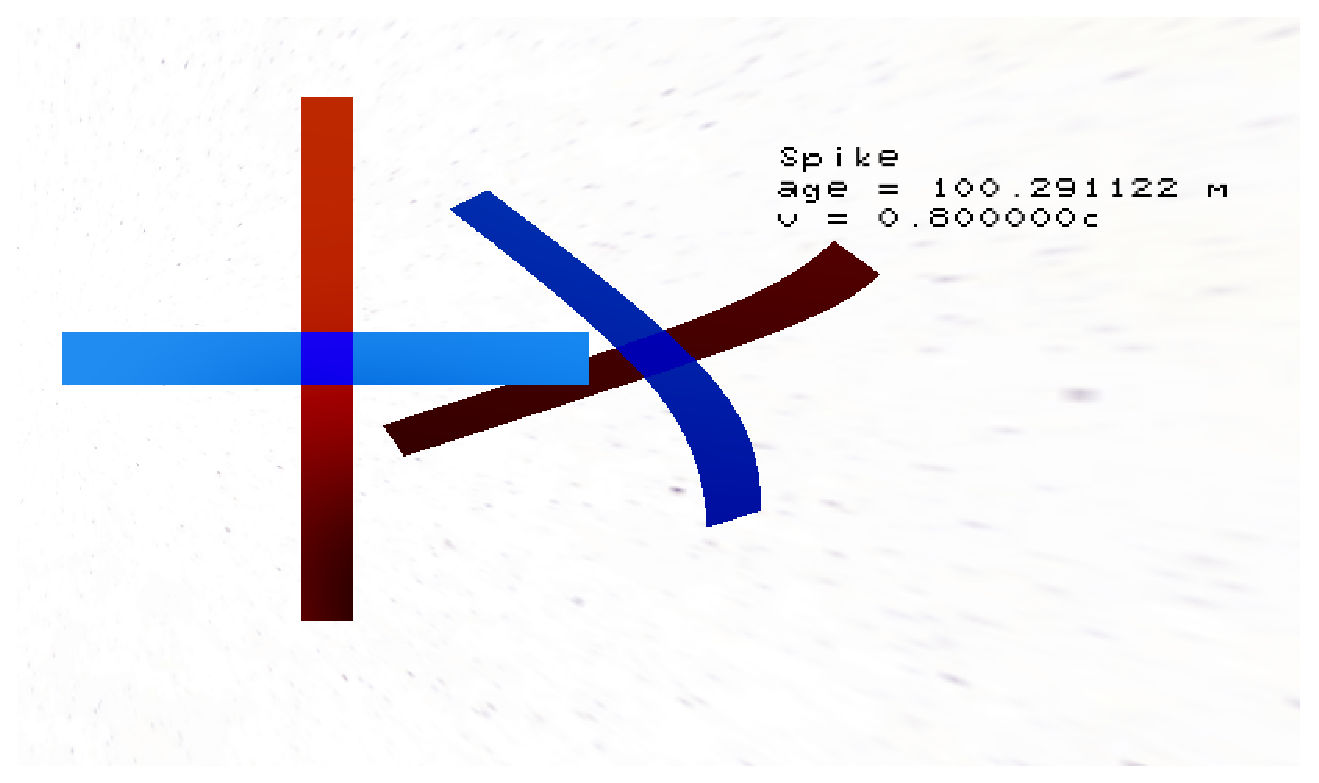
\includegraphics[width=.95\linewidth]{figures/ThomasPrecession.eps}
	% replacing the above command with the one below will explicitly set
	% the bounding box of the PS figure to the rectangle (xl,yl),(xh,yh).
  	% It will also prevent LaTeX from reading the PS file to determine
  	% the bounding box (i.e., it will speed up the compilation process)
  	% 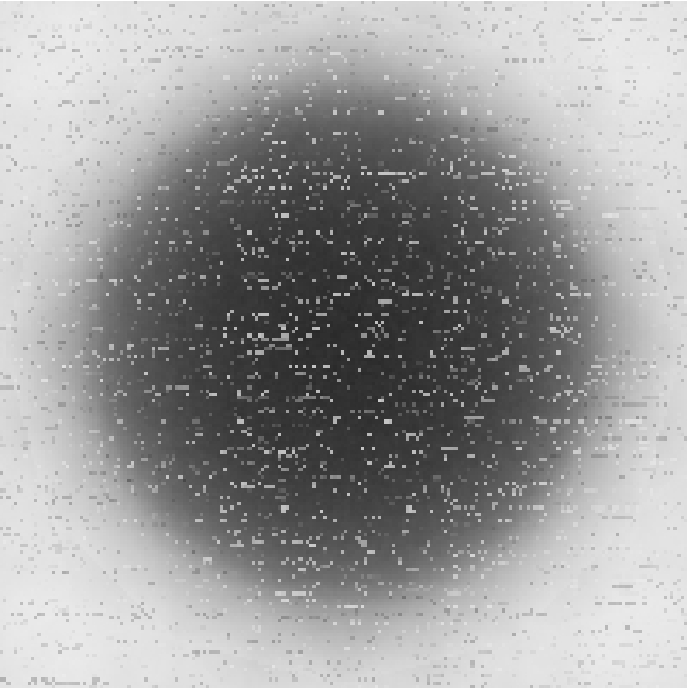
\includegraphics[width=.95\linewidth, bb=xl yl xh yh]{sampleFig.eps}
	\caption{Thomas Precession after one full rotation}
	\label{fig:thomasPrec}
\end{figure}

\FloatBarrier

\subsection{Performance}
The application implementing algorithms described in this article had been tested with different amount of detailed objects. The results of performance tests are listed in table~\ref{tab:performance}.
\begin{table}
\caption{Performance of the simulation}
\label{tab:performance}
\begin{tabular}{|r|r|r|}
\hline
Number of objects & FPS Lorentz & FPS Galilean\\
\hline
\hline
0&550&550\\
\hline
10&97&82\\
\hline
20&45&46\\
\hline
30&39&33\\
\hline
40&30&25\\
\hline
50&25&20\\
\hline
60&21&18\\
\hline
70&18&16\\
\hline
80&17&14\\
\hline
90&17&13\\
\hline
100&15&15\\
\hline
\end{tabular}

\end{table}


\section{Conclusions}
\label{sec:concl}
The methods described in this article are capable of visualisation of the most common phenomena described by the theory of special relativity. This implementation proved to be able to run with interactive frame rates while displaying detailed objects. The ability to change the parameters of the simulation enables users to experiment freely with objects moving with velocities close to the speed of light. 

\section*{Acknowledgements}
I would like to thank Dr. Nándor Bokor and Dr. László Szirmay Kalos for their valuable technical assistance and support.


\begin{thebibliography}{1}
\bibitem{EinsteinElectrodynamics} Albert Einstein.
\newblock On the Electrodynamics of Moving Bodies.
In \emph{Annalen der Physik}, \textbf{17}:891, June 1905.

\bibitem{AERelativity} Albert Einstein.
\newblock \emph{Relativity: The Special and General Theory}.
Henry Holt and company, 1920.

\bibitem{KHGalilei} Knudsen J.M., Hjorth P.G. The Galilei Transformation.
In \emph{Elements of Newtonian Mechanics}. Advanced Texts in Physics. Springer, Berlin, Heidelberg, 2000.

\bibitem{BRGPS} Buenker, Robert J.
\newblock The Global Positioning System and the Lorentz Transformation.
In \emph{Apeiron: Studies in Infinite Nature}, 15.3, 2008.

\bibitem{utkarsh} Utkarsh Bajaj.
\newblock Visual Appearance of Extended objects in Special Relativity.
\emph{arXiv}, eprint 2104.03908, April 2021.

%---------------TEMPLATES---------------------------------------
%\bibitem{yll} Y. Le Lous,
%``Report on the First Eurographics Workshop on Visualization in
%Scientific Computing'', \emph{Computer Graphics Forum\/}
%\textbf{9}(4), pp. 371--372 (December 1990).
%
%\bibitem{FolDamFeiHug.etal93}
%J. Foley, A. van Dam, S. Feiner, J. Hugues, and R. Phillips.
%\newblock \emph{Introduction to Computer Graphics}.
%\newblock Addison Wesley, 1993.
%
%\bibitem{PosFel89}
%K.Ch. Posch and D.W. Fellner.
%\newblock The Circle-Brush Algorithm.
%\newblock \emph{Transactions on Graphics}, \textbf{18}(1):1--24, 1989.
%
%\bibitem{FolHagNie93}
%T.A. Foley, H.~Hagen, and G.M. Nielson.
%\newblock Visualizing and modeling unstructured data.
%\newblock \emph{The Visual Computer}, (9):439--449, 1993.
%
%\bibitem{Lev90}
%M.~Levoy.
%\newblock Efficient ray tracing of volume data.
%\newblock \emph{ACM Transactions on Graphics},
%          \textbf{9}(3):245--261, July 1990.
%
%\bibitem{PorDuf84}
%T.~Porter and T.~Duff.
%\newblock Compositing digital images.
%\newblock \emph{ACM Computer Graphics (Proc. of SIGGRAPH '84)},
%          \textbf{18}:253--259, 1984.
%
%\bibitem{RonRos96}
%R.~Ronfard and J.~Rossignac.
%\newblock Full-range approximation of triangulated polyhedra.
%\newblock \emph{Computer Graphics Forum (Eurographics'96 Proc.)},
%          \textbf{15}(3):67--76, 1996.

\end{thebibliography}

\end{document}
%%%%%%%%%%%%%%%%%%%%%% end of EgPublSamp.tex %%%%%%%%%%%%%%%%%%%%%%
